% !TEX root = ../HDR.tex
%%%%%%%%%%%%%%%%%%%%%%%%%%%%%%%%%%%%%%%%%%%%%%%%%%%%%%%%%%%%%%%%%%%%%%%%%%%%%%%%%%
\chapter{Apprentissage spatio-séquentiel}


\section{Ontologie basée sur les affordances}

\section{Enactive Cognitive Architecture (ECA)}

\begin{figure}[ht]
	\centering
	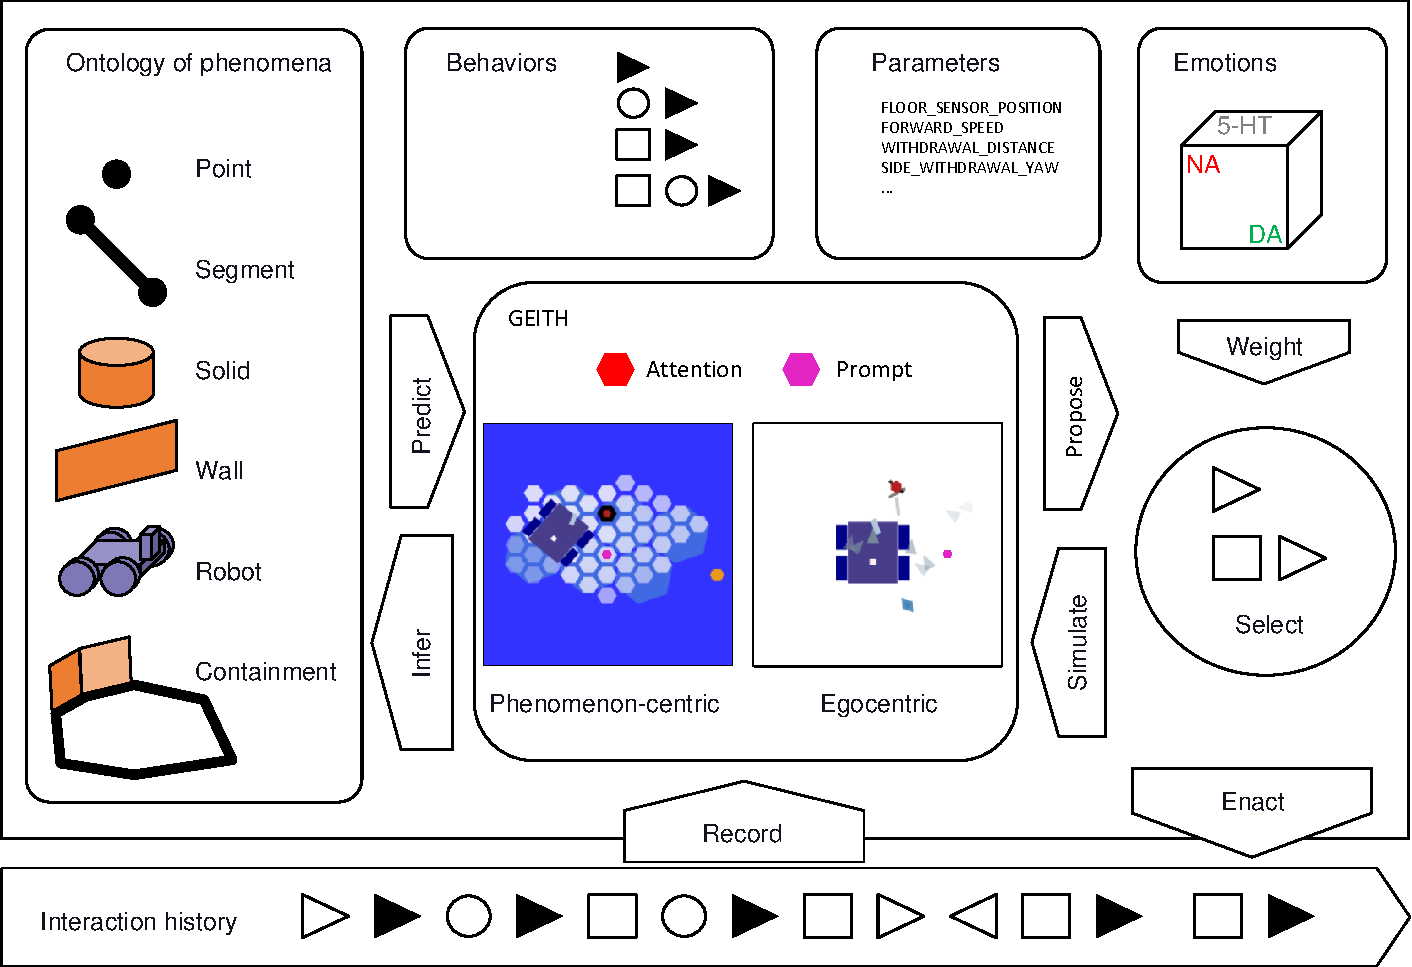
\includegraphics[width=0.6\textwidth]{Figures/5_ECA.pdf}
	\caption{The Enactive Cognitive Architecture (ECA) depuis \cite{georgeon_reducing_2024}}
	\label{fig:ECA}
\end{figure}

La Figure \ref{fig:ECA} montre la Enactive Cognitive Architecture décrite dans \cite{georgeon_reducing_2024}

